\chapter{Interactions}

Creating new interactions is a key topic for this thesis. This chapter describes the pros and cons of current state-of-the-art two-dimensional interactions and proposes improvements using the detected primitive shapes as interaction support shapes. 

Many proven interaction techniques have emerged over time, such as \textit{Point Picking} or \textit{Region Selection}. 

%% TODO: define pick ray
%% TODO: define candidate global
%% TODO: define point belongs to a shape

\section{Shape Picking}


\section{Point Picking}
\label{sec:picking}
\textit{Point Picking} describes an interaction, where the user is interested in selecting a single point from the scene at a time. A \textit{pick ray} describes a ray originating from the mouse position whose direction is the view direction. The pick radius $r$ denotes the maximum distance of a point to the pick ray in order for the point to be considered a candidate point. Depending on the use case the pick radius $r$ can be depended on the depth value. There are multiple ways of implementing this interaction with varying results. 
\\
\\
The first explored technique is to use a fixed pick radius in world space. The picked point is the point closest to the pick ray in world space. Since the user only interacts with points that are projected onto the nearplane, the projection of the pick radius is smaller for points that lie in the background. Therefore, the distance in pixel between the mouse position and a picked point in the background is smaller than the distance to a picked point in the foreground. While this encourages the picking of points in the foreground, the non-uniform pixel distance introduces inconsistencies. 
\\
\\
A more consistent way of picking a point is to only use the screen space information for each point. The mouse position $p$ in screen space combined with the pick radius $r$ create the pick circle $c$. This circle corresponds to a projection of a cone. All points that intersect this cone are treated as candidate points. In order to calculate this intersection, all points are projected to the screen space. The cone intersects a point if $c$ contains the point in screen space. Then the point with the projection closest to the mouse position is picked. This technique works consistently for different depth values. However, since all points are treated equally, the technique does not distinguish between foreground and background points, thus introducing possible depth ambiguities. 
\\
The projection of points can be executed on the GPU by rendering the projected points, paired with an identifier, to a texture. From this texture, a window around the mouse cursor is downloaded and the closest point is determined. Reading pixels from a texture forces the CPU and GPU to sync and stalls the graphics pipeline. 
\\
\\
The user interacts with points that are presented on the screen only. Moreover, only points are of interest, whose projection on the nearplane lie in close proximity to the mouse position. Since this interaction cannot be computed for all points in real-time, unneeded octree nodes must be filtered beforehand. This prefiltering can easily be achieved by performing a raycast through the octree and collecting all nodes whose bounding boxes intersect the pick ray. However, consider the case, that the pick ray does not intersect a node's bounding box, but the distance of the box to the ray is smaller than the pick radius. Some points might exist that should be considered candidates, but due to the nature of a raycast, are discarded. This introduces the possibility that points that can be the picking result, are not considered, introducing inconsistency to the pick interaction. One solution to overcome this problem is to use a conecast instead. 
\\
A circle on the nearplane is the projection of a cone in world space. The corners of the box are projected onto the nearplane and the convex hull polygon is calculated. The intersection then is determined by the intersection of the polygon with the pick circle $c$. 


\subsection{Shape-Assisted Point Picking}
Picking comes with the disadvantage that some constellations of points can influence the picking interaction in a negative way. Points that occlude structures of interest force the user to change the view in order to pick the desired point. In some cases, a point in the background is favored over a desired point on a structure. 
 \textit{Shape-Assisted Point Picking} utilizes primitive shapes to perform the picking routine only on points that are part of a structure. The user selects a cluster of shapes, thus reducing the amount of possible candidate points to only those that belong to this shape. 
\\
Instead of performing a cone- or raycast on the octree, only those nodes are taken into account, whose bounding boxes intersect the shape cluster. Each point that does not fulfill the score function from Section \ref{sec:scorefun} for the particular canidate shape is discarded as well, leaving only a handful of points on which a conecast is performed. The pick radius in world space is calculated by unprojecting the pick circle to the intersection point of the pick ray with the shape cluster. Only points are considered that lie in the pick sphere, constructed by the intersection point and the pick radius. The point closest to the intersection point is then picked. Due to the curvature of shapes, such as cylinders and spheres, points on the back of a shape are projected in close proximity to the mouse position as well. By using the projected distances, points that lie on the back side of the shape might get favored over points that are on the front side of the shape (facing the user). 
\\

This technique comes not only with interaction benefits, computation time is drastically reduced as well. Usually a shape cluster consists of less nodes than a raycast since the cluster's extension is limited to a region in the point cloud. Points within a node are also reduced such that intersections and distance measures are computed only for candidate points. 

\\
Figure \ref{fig:picking} shows the different picking methods, described in Section \ref{sec:picking}. Figure \ref{fig:picking_raycast} showcases a simple raycast with a radius. The combination of a ray and a radius yields a cylinder, which contains all candidate points on world space. The pick distance in world space is consistent. Figure \ref{fig:picking_conecast} uses a conecast instead. The opening angle is defined by the pick radius in screen space. The pick distance in world space increases the higher the depth value. All points inside the volume are treated equally, introducing consistency in screen space. \Figure\ref {fig:picking_assisted} showcases the use of a support shape to further filter candidate points. All points are filtered that belong to the support shape prior to be used as input for a spherecast. 

\begin{figure}
\centering
\subcaptionbox{ \label{fig:picking_raycast}}{%
  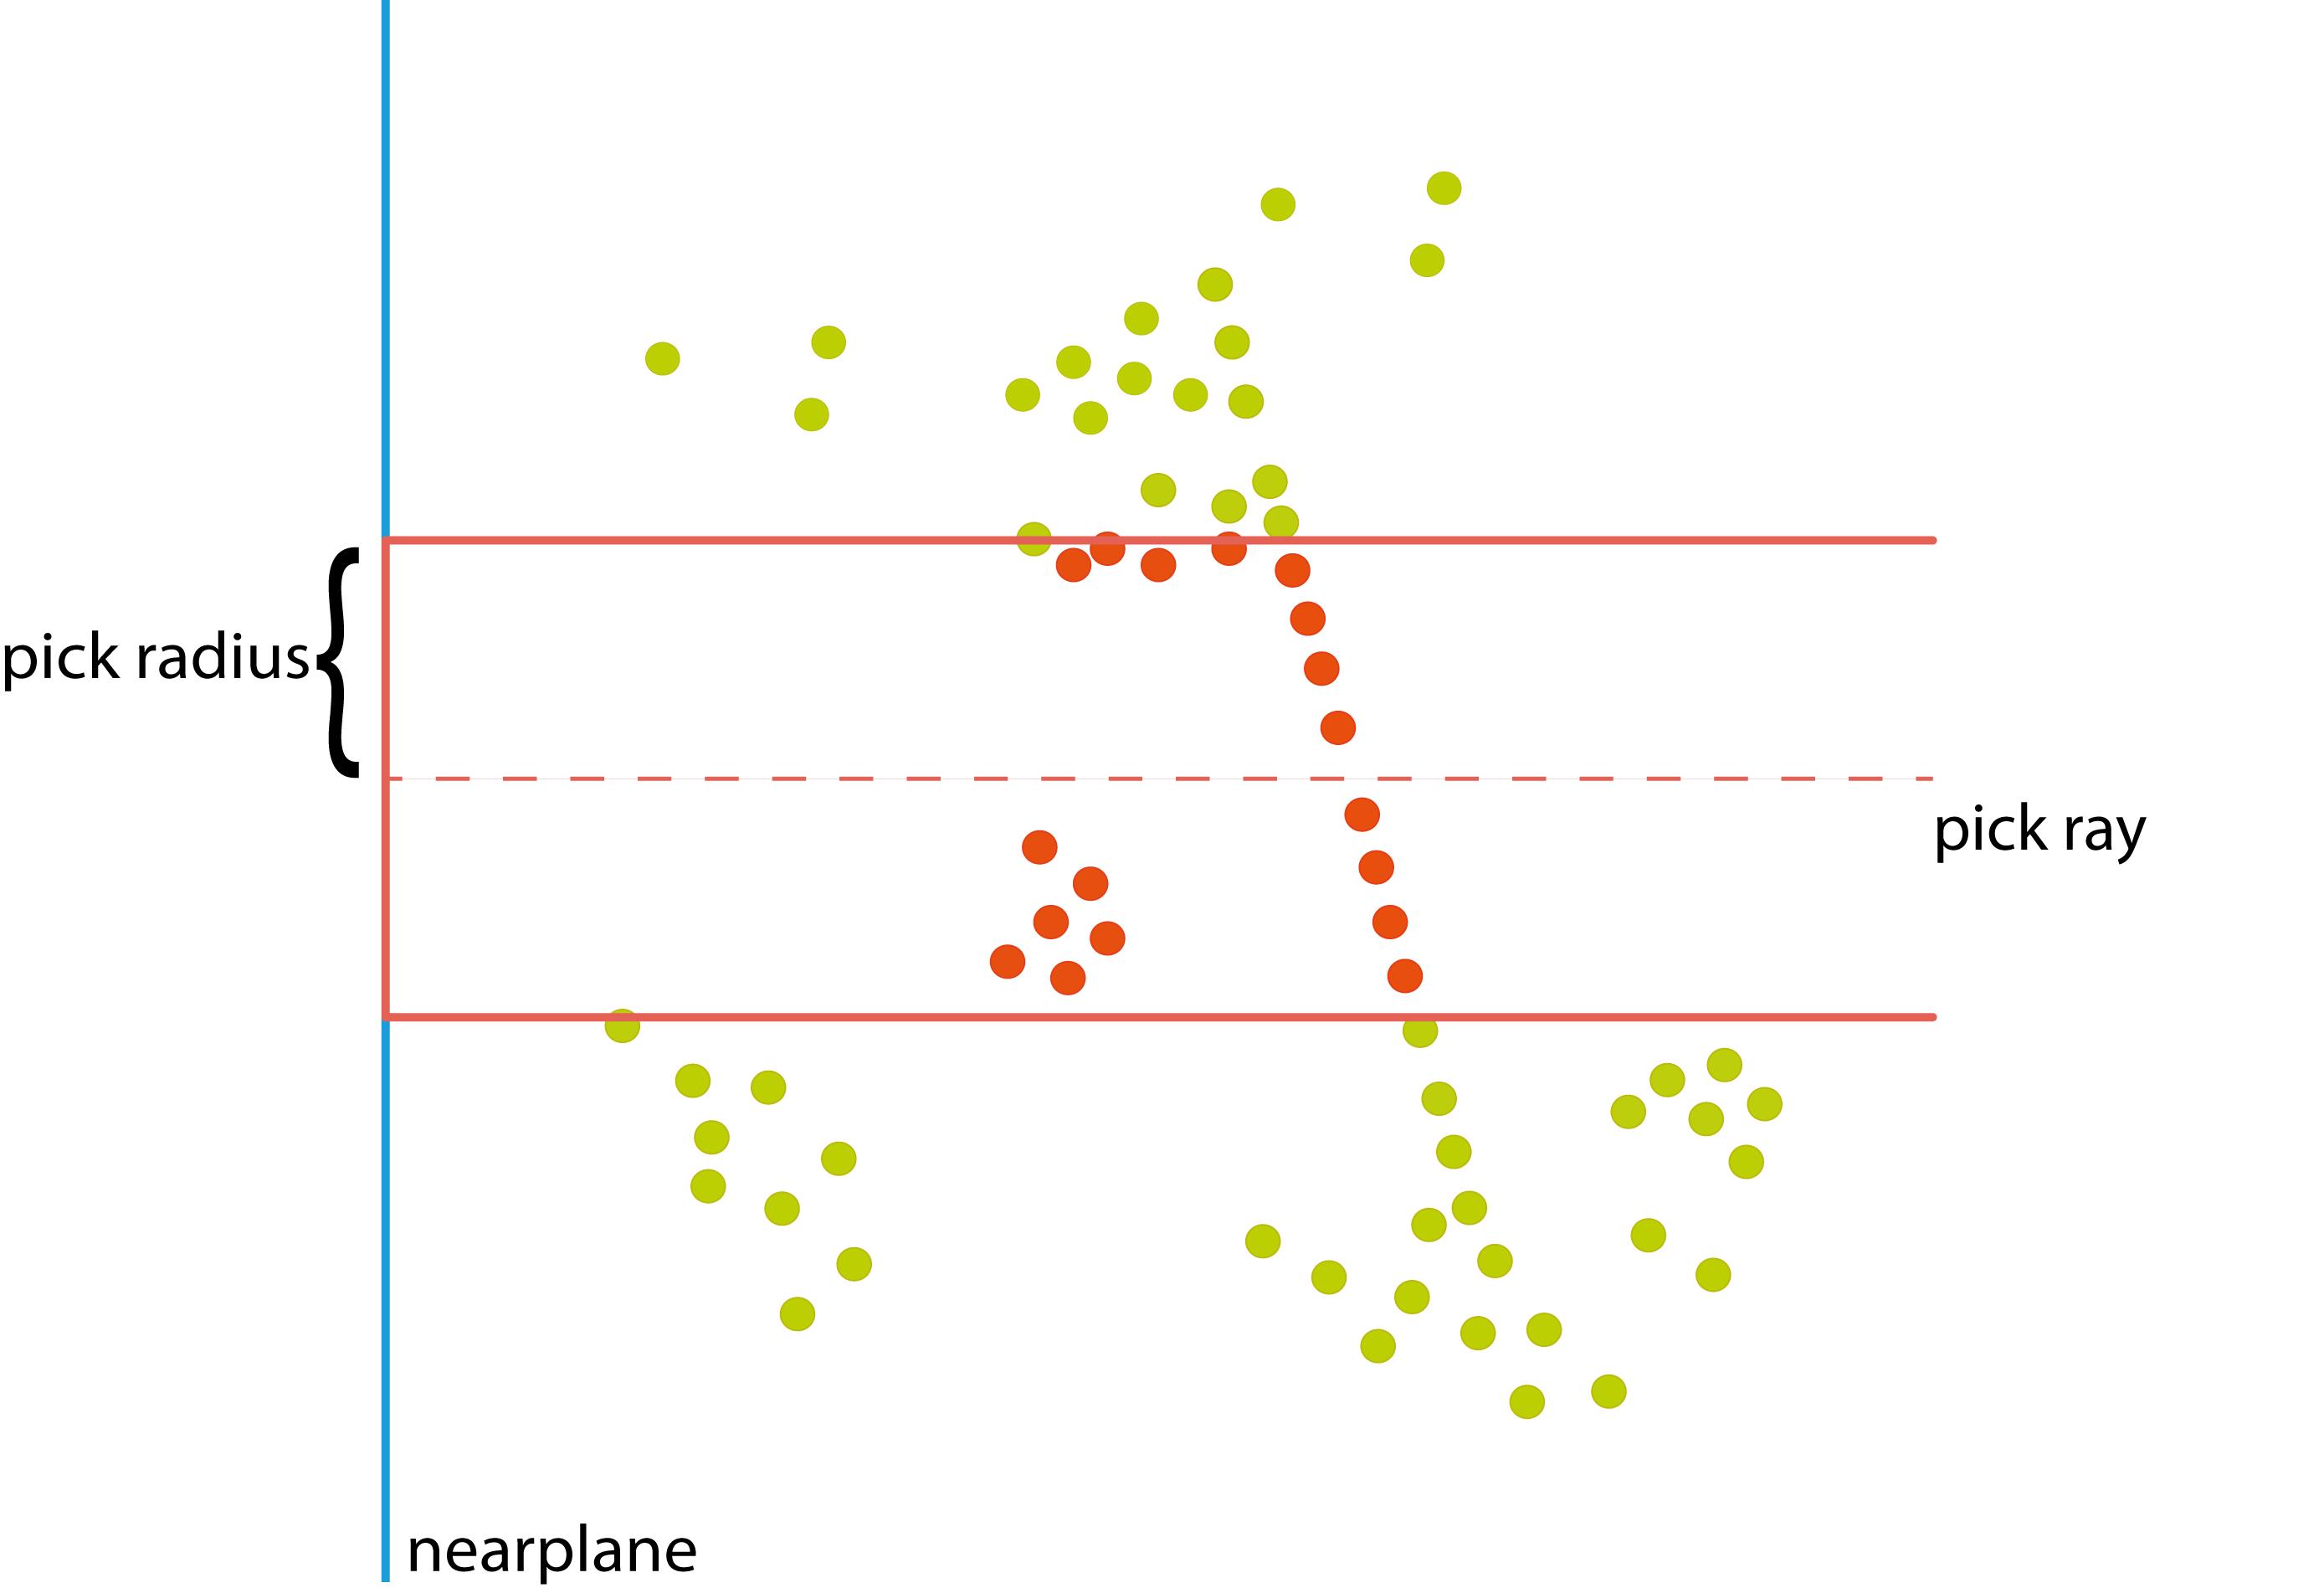
\includegraphics[width=0.6\textwidth]{Interactions/picking_raycast.png}%7
  }\par\medskip
\subcaptionbox{ \label{fig:picking_conecast}}{%
  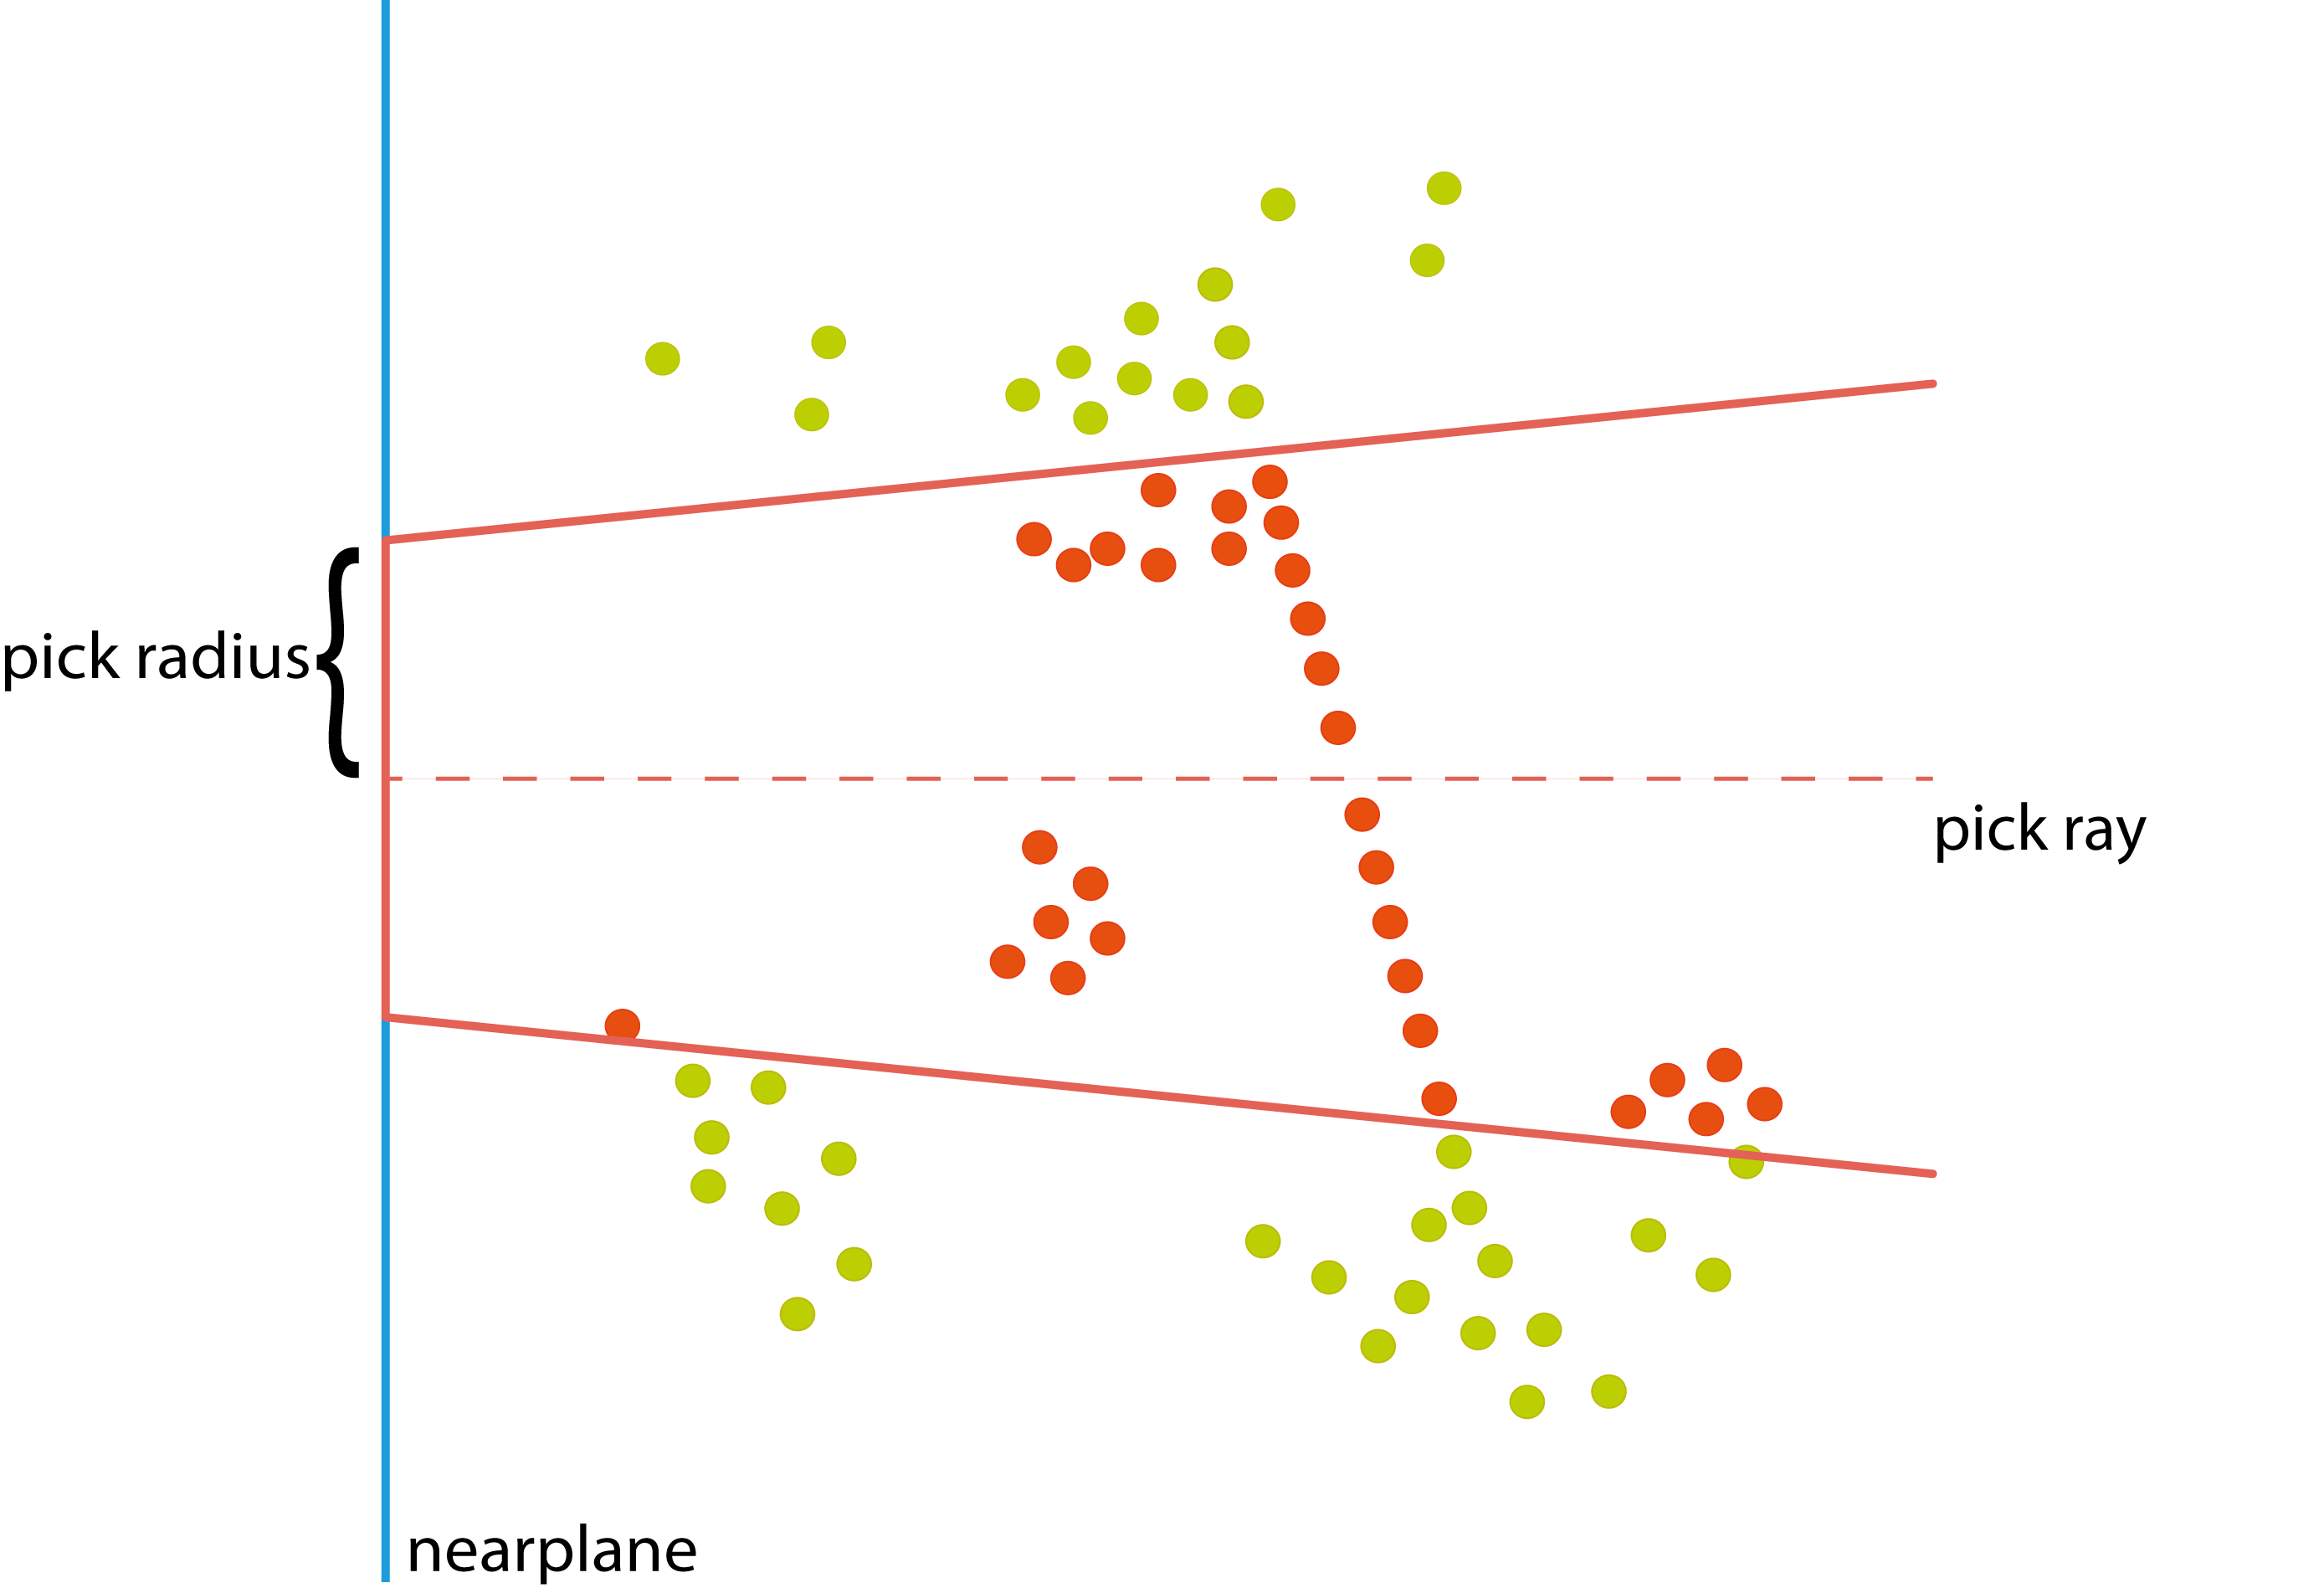
\includegraphics[width=0.6\textwidth]{Interactions/picking_conecast.png}%
  }\par\medskip        
\subcaptionbox{ \label{fig:picking_assisted}}{%
  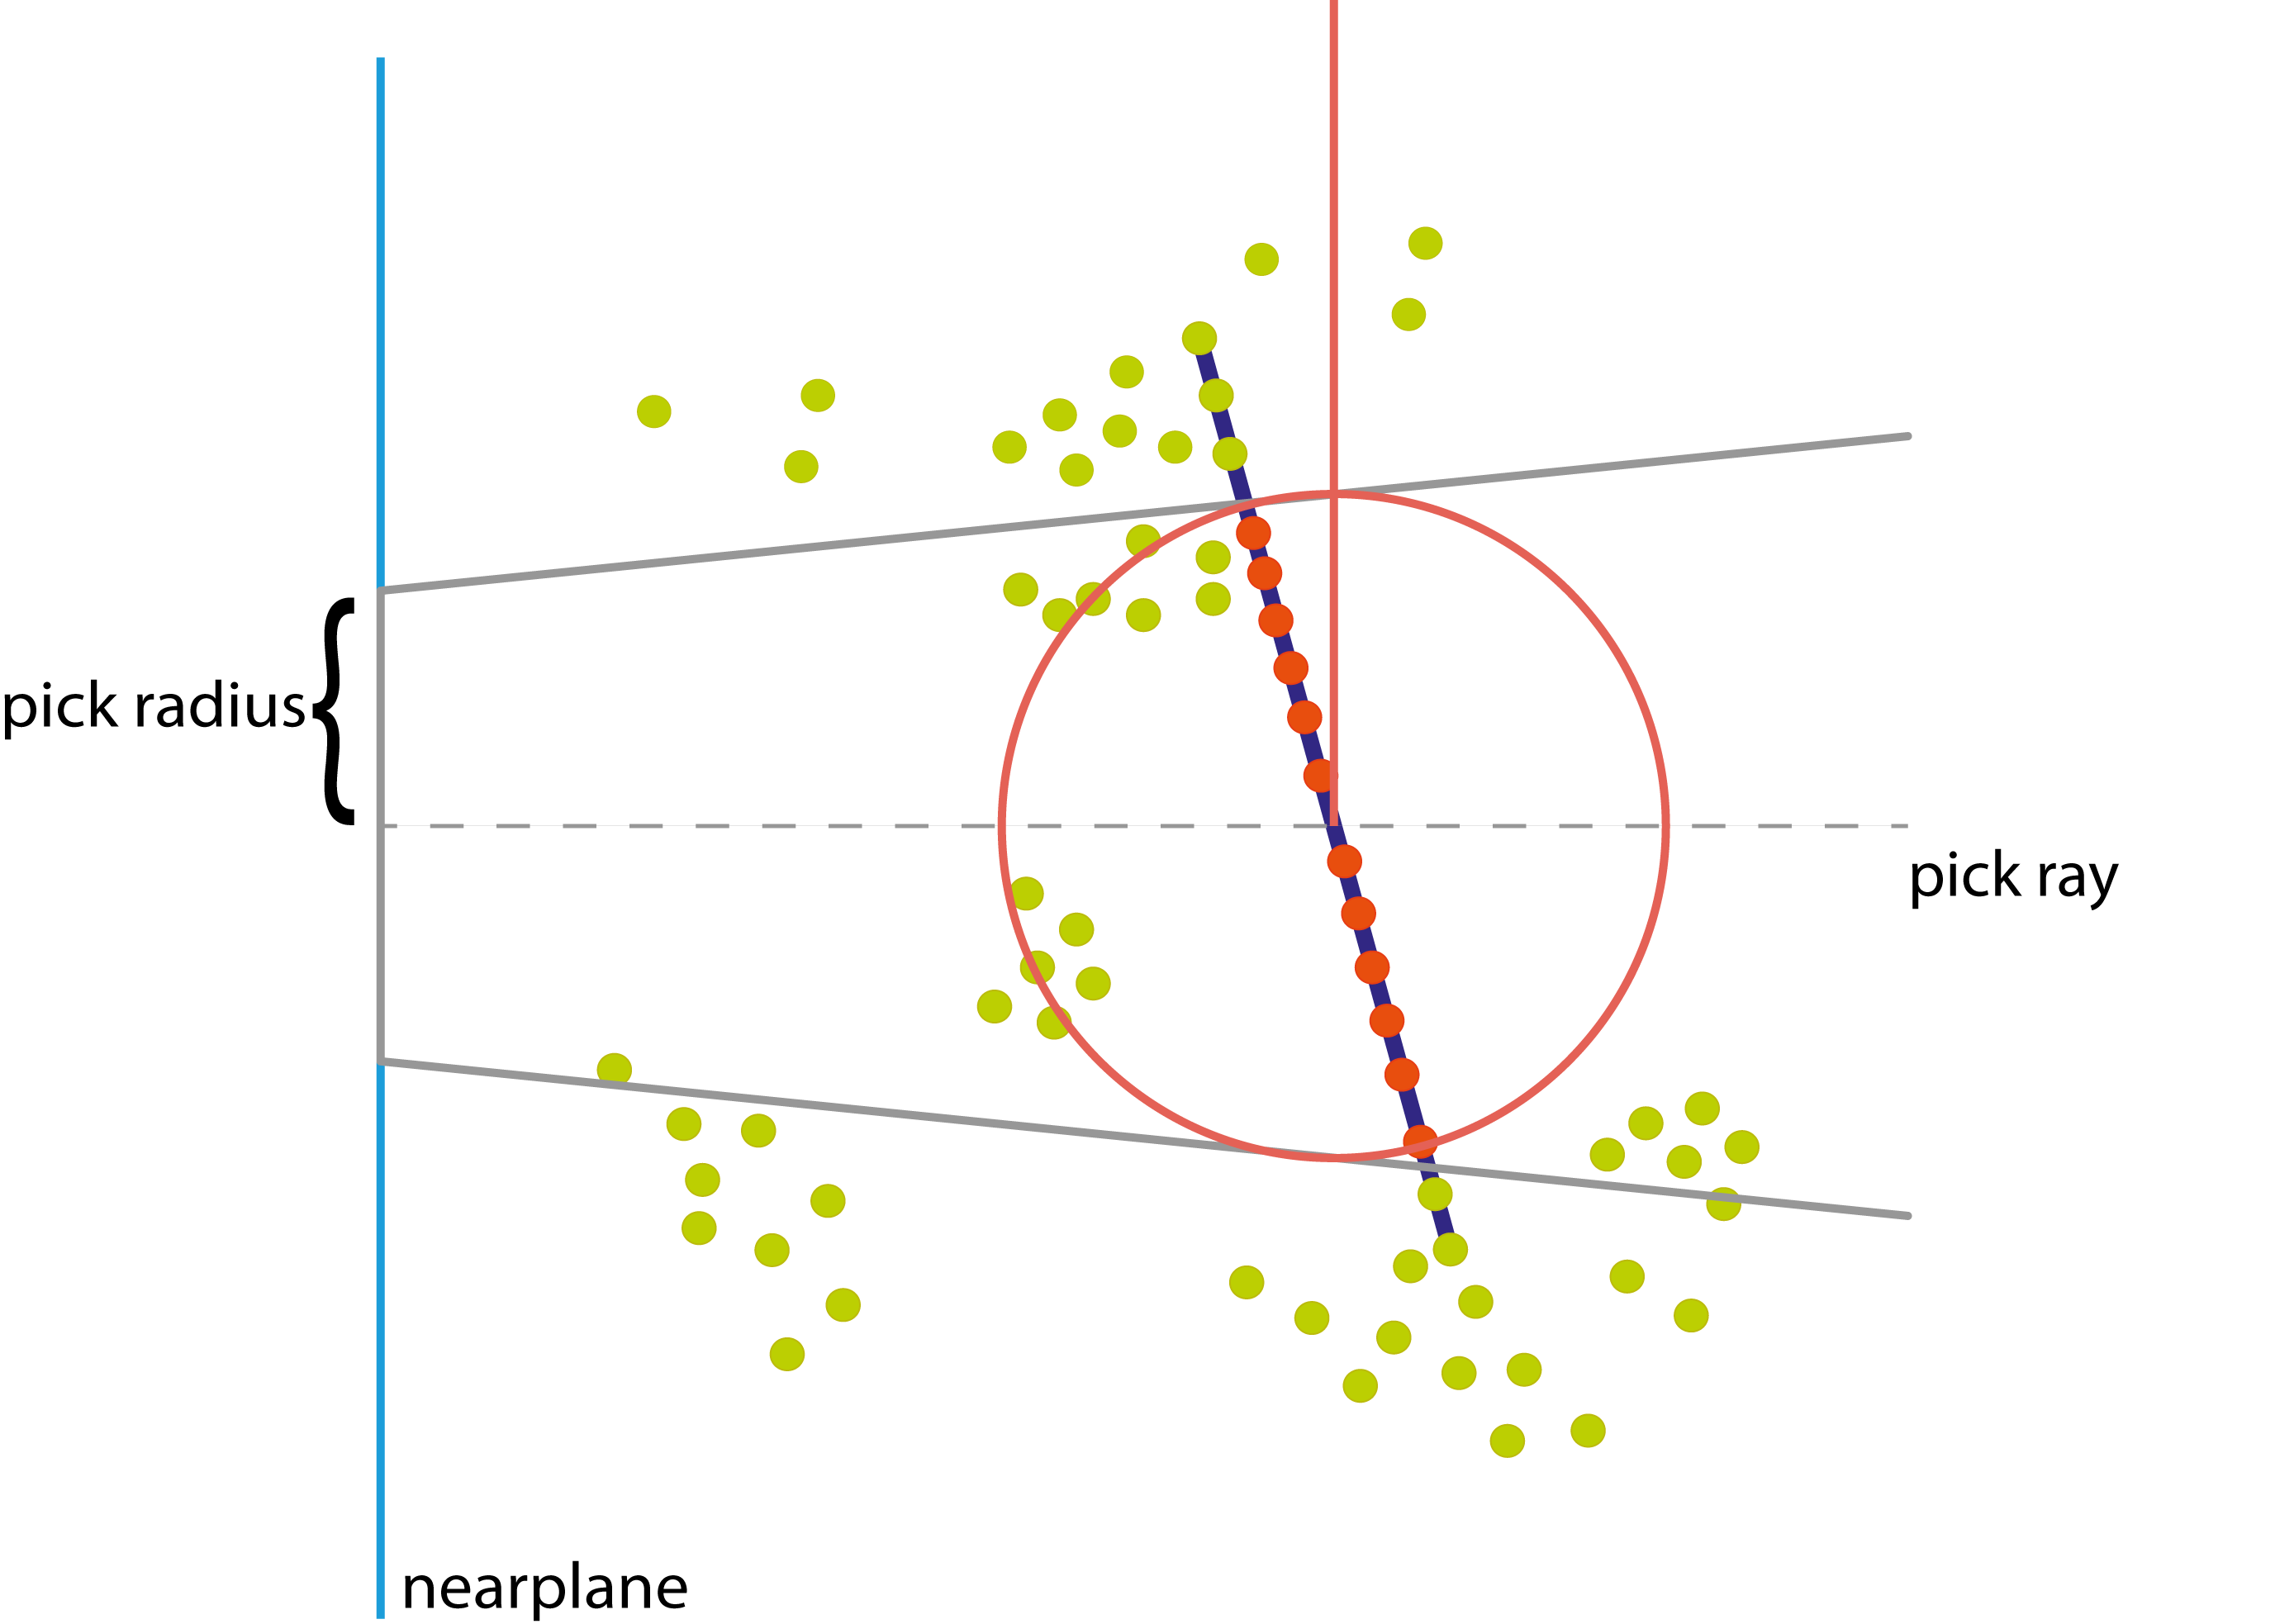
\includegraphics[width=0.6\textwidth]{Interactions/picking_assisted.png}%
  }
\caption{Two-dimensional illustration of various picking methods. Candidate points are colored in green, other points are colored in red. The areas in red describe the different volumes in which candidate points are located. (a) showcases a picking process using a simple raycast. The ray combined with a radius constructs a cylinder in world space which contains all candidate points, (b) uses a cone instead. (c) utilizes a selected shape (dark blue) in order to further filter the candidate points to only follow the curvature of the shape. A spherecast is then performed on the filtered points using the unprojected pick radius as radius to select the final set of candidate points. }
\label{fig:picking}
\end{figure}


\section{Region Selection}

Region Selection aims to not pick a single point at once, but select a set of points, that are spatial neighbors
The design for the \textit{Shape-Assisted Region Selection} is guided by one seemingly simple example task: \textit{Select points that belong to this wall only}. A wall can intersect with other building elements such as roof, balconies or the ground. In regions close to intersections, it is tedious and cumbersome to only select points on the desired structure. Using two-dimensional interaction metaphors, selecting spatially neighboring points along the same curvature, is particularly challenging, since the system does not know the desired depth boundaries for the selection region. In this chapter the benefits of using support shapes for two- and three-dimensional interaction metaphor are discussed. 


\subsection{Volumetric Brush}

The \textit{Volumetric Brush} by Weyrich et. al\cite{weyrich2004post} is designed in such a way that a volume is projected onto the foremost geometry. Points that intersect this volume are considered to be selected. To retrieve the projected position of the volume, usually a sphere, the depth buffer is consulted and the depth value for the current mouse position is retrieved. The world position is the unprojection of the mouse position's $xy$-coordinates and the depth value. 
\\
Since this technique follows the foremost geometry only, sudden depth changes occur if the area of interest is occluded by different geometry. Thus view changes are still required to achieve the example task. In regions close to intersections with other structures, such as below the roof, the user must control the size of the volume in order to not select points on neighboring structures. 


\subsection{Lasso Selection}

The \textit{Lasso Selection} is a common two-dimensional interaction metaphor used for multiple geometry-based applications. While it is an effective technique to selected regions in 2D, drawbacks appear when porting the interaction to 3D. The user draws a polygon onto the screen. All points, whose projection lie inside this polygon, are selected. Much like \textit{Point Picking}, points are projected onto the nearplane and and the intersection between the point and the polygon determines if the point is selected. The combination of a two-dimensional polygon and the projection of points describes an three-dimensional area. The polygon is extruded in the view direction up to a user-defined distance. All points that lie within this volume are selected. Figure \ref{fig:lasso_sketch} showcases the volume created by a lasso polygon drawn onto the screen.


\begin{figure}
	\centering
	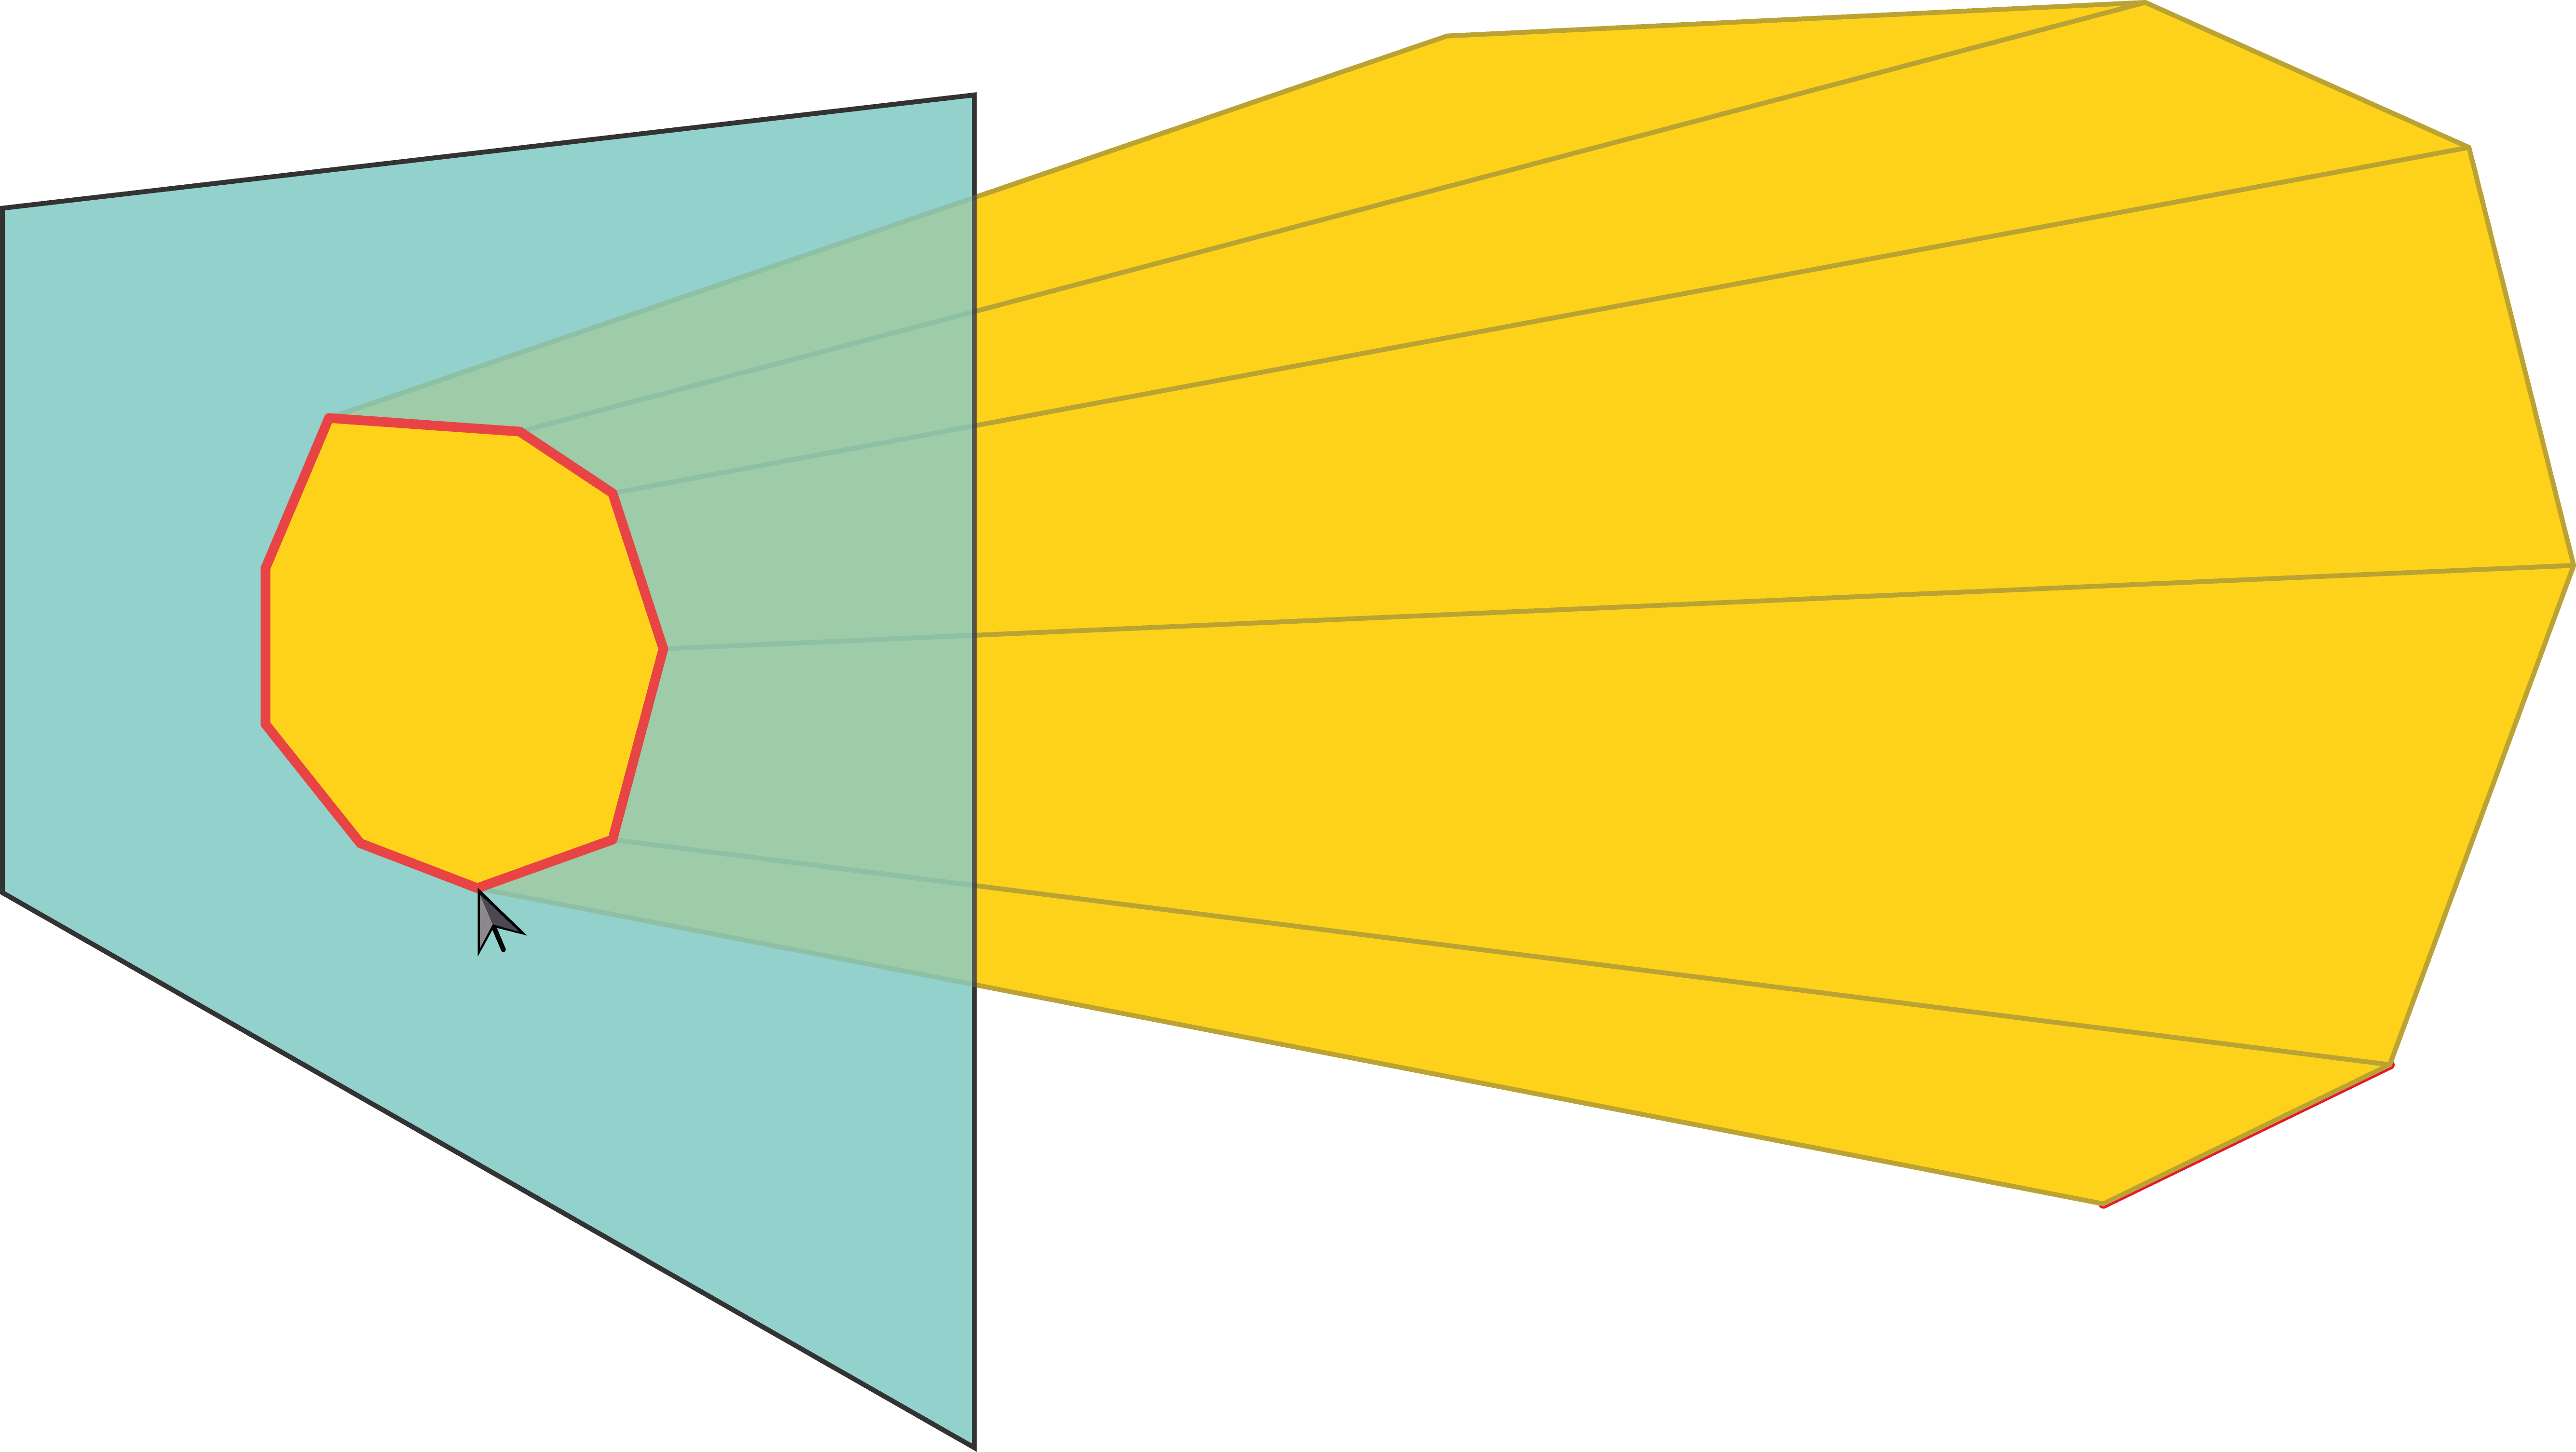
\includegraphics[width=0.8\textwidth]{Interactions/lasso_sketch.png}%7
	\caption{The user draws a polygon(red) on the screen(light blue). The constructed three-dimensional area(yellow) contains all points, whose projection lie inside the lasso polygon. }
	\label{fig:lasso_sketch}
\end{figure}


\begin{figure}
\centering
\subcaptionbox{ \label{fig:lasso1}}{%
  \includegraphics[width=0.5\textwidth]{Interactions/lasso1.png}%7
  }\par\medskip
\subcaptionbox{ \label{fig:lasso2}}{%
  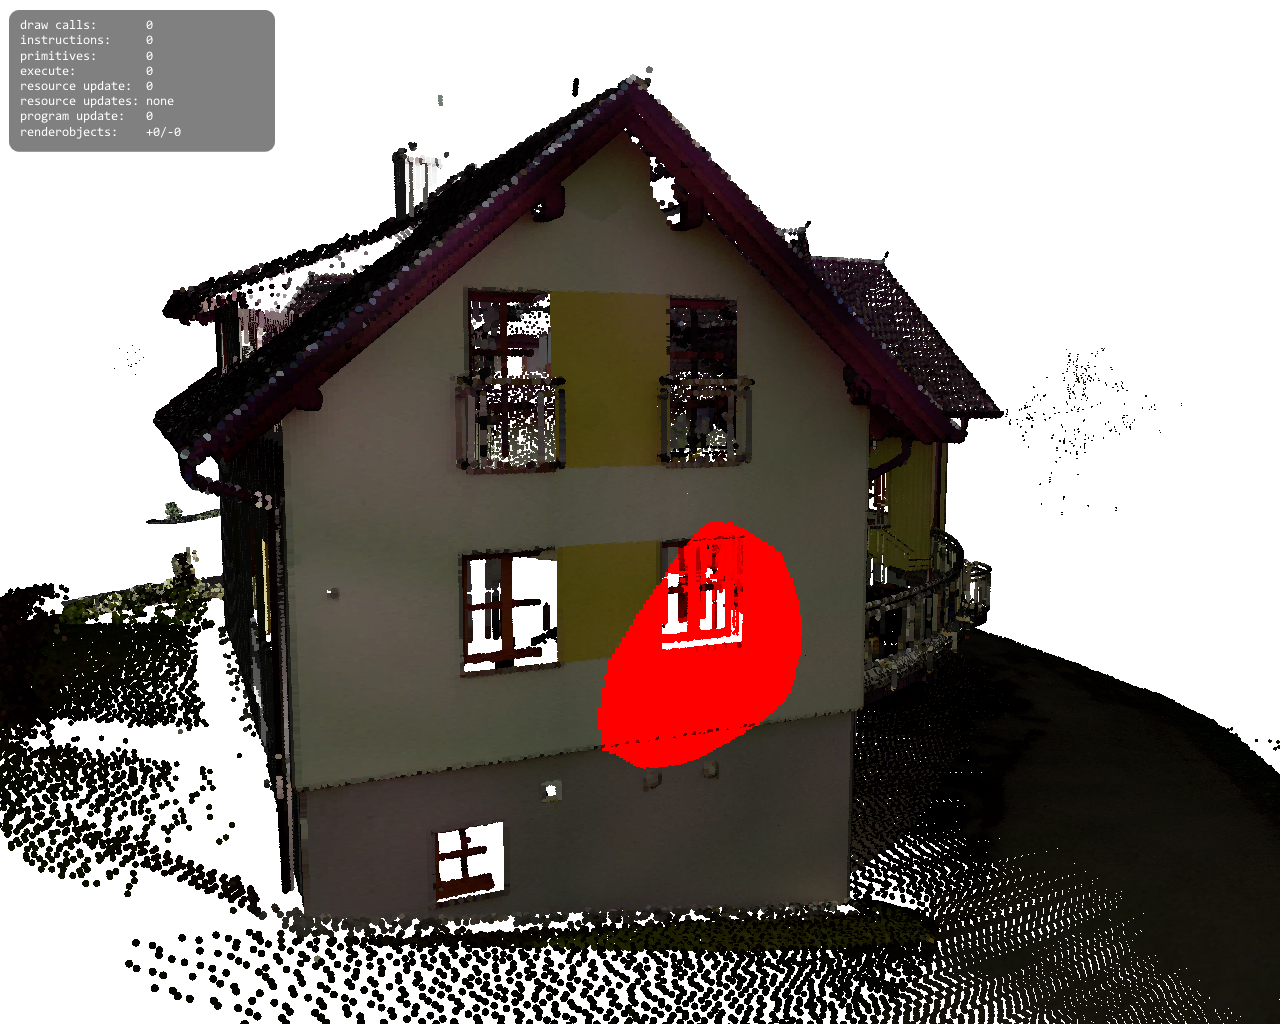
\includegraphics[width=0.5\textwidth]{Interactions/lasso2.png}%
  }\par\medskip        
\subcaptionbox{ \label{fig:lasso3}}{%
  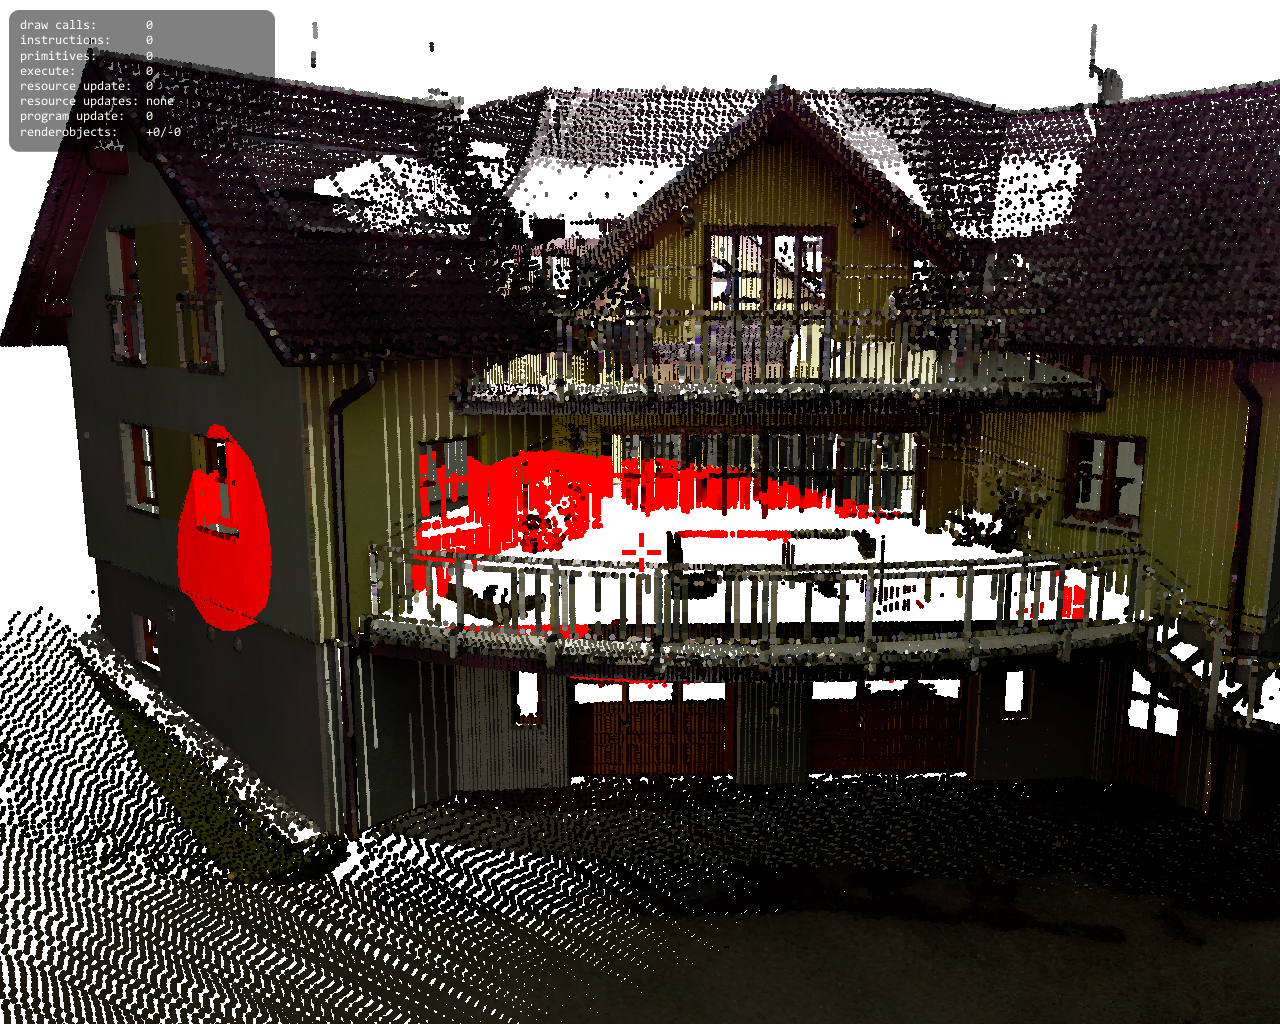
\includegraphics[width=0.5\textwidth]{Interactions/lasso3.png}%
  }
	
\caption{(a) - (c) show a lasso selection performed on a point cloud. In (a) the user draws a polygon onto the screen. In (b) the selected points are visualized in red. Figure (c) showcases the selection from a different angle. All points that are projected to the area of the polygon, are selected. This results in the unintentional selection of points that are obscured by objects in the foreground.}
\label{fig:lasso}
\end{figure}


Figure \ref{fig:lasso} shows a lasso selection performed on a point cloud. The user draws a polygon onto the screen. The selected points are highlighted in red. When changing the view, selected points that where occluded when drawing the lasso, appear. The user must control the selection distance by hand in order to minimize this effect. However, the in order to solve the task of only selecting points on the wall, further lasso selections must be used to remove points from the selection that where selected unintentionally. 





\subsection{Shape-Assisted Region Selection}
\section{Shape-Assisted Local Level-of-Detail Increase}
